\documentclass[10pt,border=1pt]{standalone}
\usepackage[T1]{fontenc}
\usepackage{mathpazo}
\usepackage{amsmath,amssymb}
\usepackage{xcolor}
\usepackage{pgfplots}
\pgfplotsset{compat=1.18}
\usetikzlibrary{shapes.geometric,positioning,arrows.meta,calc}
\definecolor{okorange}{HTML}{E69F00}
\definecolor{oksky}{HTML}{56B4E9}
\definecolor{okgreen}{HTML}{009E73}
\definecolor{okblue}{HTML}{0072B2}
\definecolor{okverm}{HTML}{D55E00}
\definecolor{okpurple}{HTML}{CC79A7}
\colorlet{accent}{okverm}
\pgfplotsset{
  safenest/.style={
    tick label style={font=\footnotesize},
    label style={font=\small},
    title style={font=\small, align=left},
    legend style={font=\footnotesize, draw=none, fill=none, cells={anchor=west}},
    grid style={black!12, line width=0.3pt},
    axis line style={black!70, line width=0.4pt},
    tick style={black!70, line width=0.4pt},
    axis lines*=left,
  },
}
\newlength{\figwidth}
\tikzset{every node/.append style={execute at begin node={\hyphenpenalty=10000\exhyphenpenalty=10000\relax}}}
\setlength{\figwidth}{18.47cm}
\begin{document}
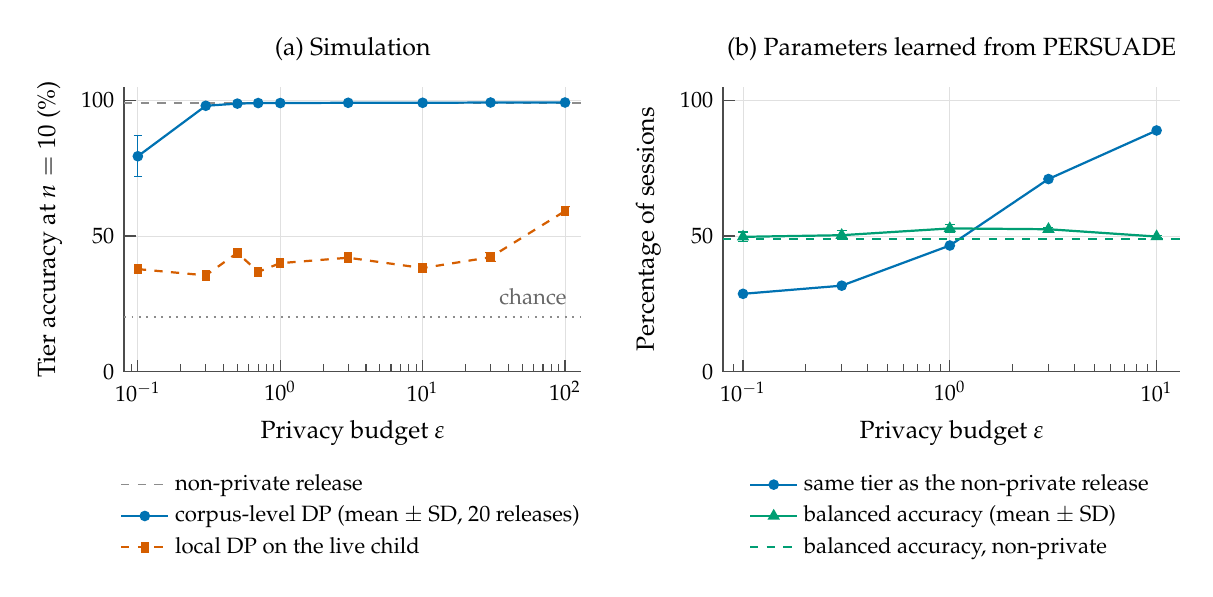
\begin{tikzpicture}
\begin{axis}[safenest, name=l, width=0.40\figwidth, height=52mm,
  xmode=log, log basis x=10, xmin=0.08, xmax=130, ymin=0, ymax=105,
  xlabel={Privacy budget $\varepsilon$}, ylabel={Tier accuracy at $n=10$ (\%)},
  xmajorgrids, ymajorgrids, title={(a) Simulation},
  legend style={at={(0.5,-0.32)}, anchor=north, legend columns=1},
]
\addplot[black!45, dashed, line width=0.6pt] coordinates {(0.08,99.0) (130,99.0)};
\addlegendentry{non-private release}
\addplot[mark=*, mark size=1.5pt, okblue, line width=0.8pt,
  error bars/.cd, y dir=both, y explicit, error bar style={line width=0.4pt}]
  coordinates {(0.1,79.4) +- (0,7.6) (0.3,98.0) +- (0,0.7) (0.5,98.8) +- (0,0.5) (0.7,99.0) +- (0,0.5) (1.0,99.0) +- (0,0.5) (3.0,99.1) +- (0,0.5) (10.0,99.1) +- (0,0.3) (30.0,99.2) +- (0,0.5) (100.0,99.2) +- (0,0.5)};
\addlegendentry{corpus-level DP (mean $\pm$ SD, 20 releases)}
\addplot[mark=square*, mark size=1.5pt, accent, dashed, line width=0.8pt]
  coordinates {(0.1,37.8) (0.3,35.5) (0.5,43.8) (0.7,36.8) (1.0,40.0) (3.0,42.0) (10.0,38.2) (30.0,42.2) (100.0,59.2)};
\addlegendentry{local DP on the live child}
\addplot[black!45, dotted, line width=0.7pt, forget plot] coordinates {(0.08,20) (130,20)};
\node[font=\footnotesize, anchor=south east, text=black!60] at (axis cs:120,21) {chance};
\end{axis}
\begin{axis}[safenest, name=r, at={($(l.east)+(18mm,0)$)}, anchor=west,
  width=0.40\figwidth, height=52mm,
  xmode=log, log basis x=10, xmin=0.08, xmax=13, ymin=0, ymax=105,
  xlabel={Privacy budget $\varepsilon$}, ylabel={Percentage of sessions},
  xmajorgrids, ymajorgrids, title={(b) Parameters learned from PERSUADE},
  legend style={at={(0.5,-0.32)}, anchor=north, legend columns=1},
]
\addplot[mark=*, mark size=1.5pt, okblue, line width=0.8pt] coordinates {(0.1,28.7) (0.3,31.7) (1.0,46.5) (3.0,71.0) (10.0,88.9)};
\addlegendentry{same tier as the non-private release}
\addplot[mark=triangle*, mark size=1.8pt, okgreen, line width=0.8pt,
  error bars/.cd, y dir=both, y explicit, error bar style={line width=0.4pt}]
  coordinates {(0.1,49.7) +- (0,1.8) (0.3,50.3) +- (0,1.7) (1.0,52.8) +- (0,1.3) (3.0,52.5) +- (0,0.7) (10.0,49.8) +- (0,0.5)};
\addlegendentry{balanced accuracy (mean $\pm$ SD)}
\addplot[okgreen, dashed, line width=0.6pt] coordinates {(0.08,48.9) (13,48.9)};
\addlegendentry{balanced accuracy, non-private}
\end{axis}\end{tikzpicture}
\end{document}
